\chapter{GAT-Denoiser}
\label{sec:contribution}

In this chapter, I will introduce my methodological approach.
As a result, a GNN is derived which is called \textit{GAT-Denoiser}.
Its main components and overall architecture are introduced.
GAT-Denoiser is implemented for 2D CT and therefore, some details for the 2D case are given.


\paragraph{Goal:}
CT and Cryo-EM in the high-noise regime is the domain of interest.
For a given set of observations, a denoising model is sought, while
it enables denoising of observations such that reconstruction quality increases.
As a first step toward an algorithm that works for unknown observation angles, 
angles are fixed during the practical part of this Thesis.


\paragraph{Input Graph:}
As $\theta$ is fixed, angles corresponding to each observation are known.
Therefore, a graph can be constructed to model neighboring observations 
based on their angles.
To define a distance measure, angles can be mapped to the unit circle (or sphere).
Then, a geodesic distance can be computed with the great-circle distance.
Based one these distances, a k-NN graph can be constructed.


\begin{tcolorbox}[colback=red!5!white,colframe=red!75!black]
  For GAT-Denoiser with fixed angles, this entails that graph topology is fixed and
  a k-NN graph can be constructed from $\theta$.
\end{tcolorbox}

\section{Pipeline}
\label{sec:concept}
The GAT-Denoiser pipeline consists of three neural network parts, namely convolution, GAT and U-Net.
For readers who are not familiar with these concepts, Appendix~\ref{sec:neural_networks} presents an introduction.

GAT-Denoiser is a GNN and has two main components, namely convolution layers and GAT layers.
The main idea of GAT-Denoiser is to enable denoising of observations:
\begin{equation}
  \textit{GAT-Denoiser} (\cdot) : \mathbb{R}^{N \times M} \to  \mathbb{R}^{N \times M} , y \mapsto \textit{GAT-Denoiser} (y) 
\end{equation}

% The GAT is expected to denoise observation signal with its neighbours by averaging. 
% Further, convolution is added to denoise single observations.

Input $y$ of GAT-Denoiser is a noisy observation and the output is a denoised version.
GAT averages over observation neighbors and convolution denoise single observations. 
For every GAT layer there is a preceding convolution. 
In the case of CT, convolution is in 1D, where for Cryo-EM it is in 2D.

\begin{tcolorbox}[colback=red!5!white,colframe=red!75!black]
  The GAT denoise observation signal with its neighbors by averaging. 
  Further, convolution is added to denoise single observations.
\end{tcolorbox}

In Figure~\ref{fig:overall-concept} the GAT-Denoiser pipeline is illustrated.
But, the main overall goal is to get the best possible reconstruction $x^{\prime}$ 
from noisy observation $y$ which approximates biological sample $x$ and 
not just denoise observation $y$ which approximates noiseless observation $p$.


\begin{equation}
  \begin{aligned}
    x \approx   &\textit{Recon} \left( \textit{GAT-Denoiser} \left( y \right) \right) = x^{\prime} \\
  \end{aligned}
\end{equation}

Therefore, an end-to-end learning approach is used where quality of reconstruction is 
compared during GAT-Denoiser training, which is expected to perform better than 
only optimizing denoising of observations.

\begin{figure}[H]
  \centering
  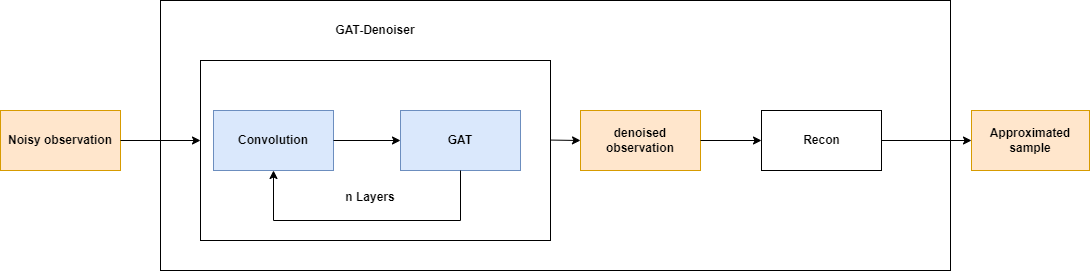
\includegraphics[width=\textwidth]{Overall_GAT-Denoiser_Pipeline.drawio.png}
  \caption{GAT-Denoiser pipeline.}
  \label{fig:overall-concept}
\end{figure}


\section{Layers}
The input to the neural network layers are observations and output are denoised observations.
Therefore, input and output dimension is defined as  $\mathbb{R}^{N \times M}$. 

Figure~\ref{fig:architecture-detailed} presents the detailed GNN architecture.
It is parametrized with $channels$, $heads$ and $layers$. 
The number of channels in convolution can be increased with parameter $channels$.
Further, $heads$ determines the number of heads used in the GAT layers and parameter 
$layers$ defines how many convolution and GAT layers are stacked together.

\begin{figure}[H]
  \centering
  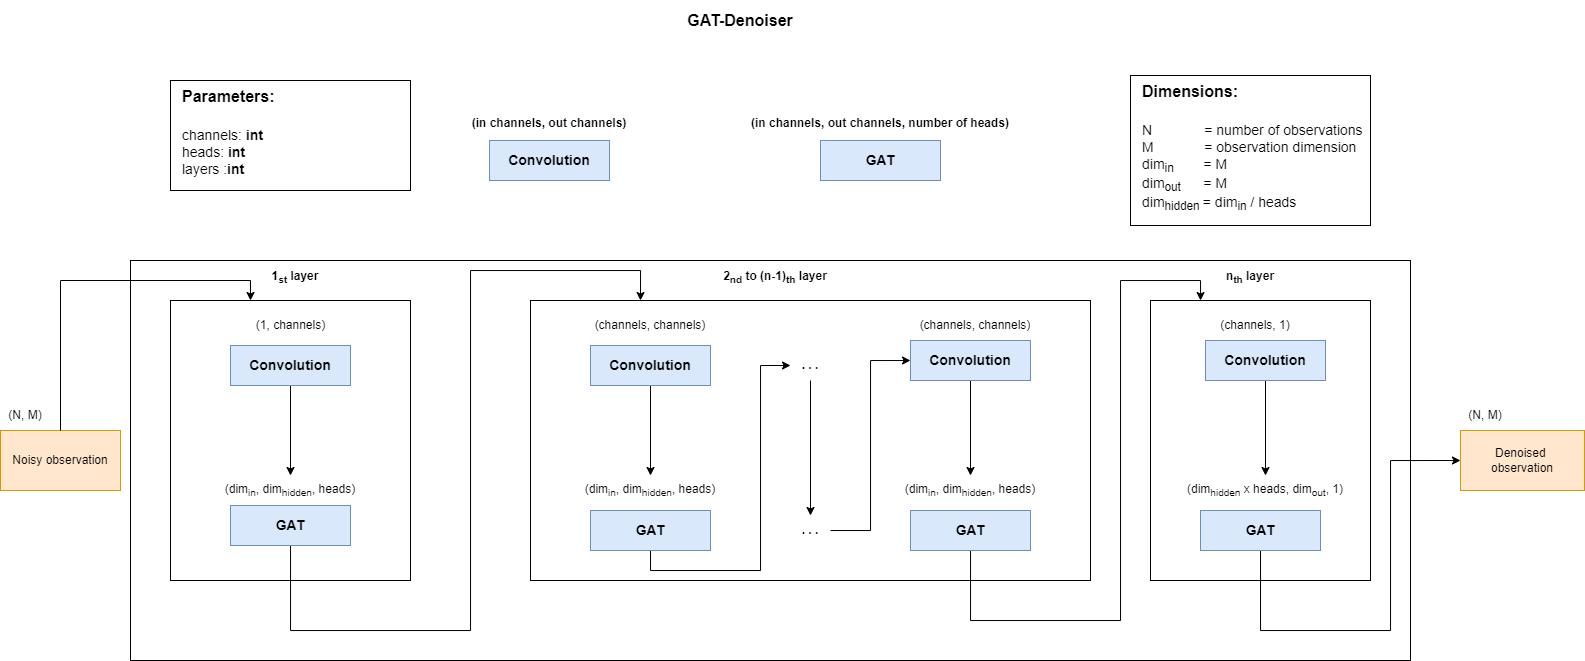
\includegraphics[width=\textwidth]{GAT_Architecture_Detail.drawio.png}
  \caption{GAT-Denoiser layers.}
  \label{fig:architecture-detailed}
\end{figure}


For every layer, first convolution and then GAT is processed. 
As input and output dimension is the same for GAT-Denoiser,
convolution needs to be defined, such that the size of the input signal needs to be the same as the size of the input signal
(e.g. kernel size 3 and padding 1).
Further, additional convolutional channels can be used for learning.
If parameter $channels > 1$, channels are increased in the first convolution layer 
and decreased in the last one.
Parameter $heads$ controls the multi-head approach of GAT. The input and hidden dimension
of GAT is $M$, when no heads are applied.
If multi-head attention is applied, hidden dimension will be set to $\frac{M}{heads}$.
In the last GAT layer, everything gets prepared for output dimension and 
averaging with 1 head is applied.

\paragraph{K-hop Neighborhood:}
In GNNs, multiple layers expose the k-hop neighborhood. Thus, for a network with $k$ layers,
the network operates in the $k$-hop neighborhood. In GAT-Denoiser, this corresponds
to the layers of GAT.

\section{Training}

For GAT-Denoiser, one could think of two different losses to use during training.
First, the loss could be defined on an observation level, what is denoted by $\mathcal{L}_{sino}$. 
The $\ell2$-norm is giving a meaningful measure:

\begin{equation}
  \label{eq:loss_sino}
  \mathcal{L}_{sino} = \parallel p - \textit{GAT-Denoiser}(A(x, \theta, s) + \eta) \parallel ^2_2
\end{equation}

Second idea is to use an end-to-end learning approach where quality of reconstruction is 
compared in the loss. Thus, the output of GAT-Denoiser is not directly part of the loss, but first reconstruction will be computed.
As the quality of the reconstruction is measured in the loss, resulting model is expected to be optimized
for reconstruction quality, and not observation quality. But, it is expected to be more computing expensive,
as reconstruction is needed to calculate loss during training.

\begin{equation}
  \label{eq:loss_reco}
  \mathcal{L} = \parallel x - \textit{Recon} ( \textit{GAT-Denoiser}(A(x, \theta, s) + \eta)) \parallel ^2_2
\end{equation}

Access to biological sample $x$ or clean observation $p$ is required during training.

\paragraph{Dropout:}
Dropout is used in neural network for regularization, thus to prevent over fitting. 
During training the neural network, some units are randomly omitted. Therefore, the network is 
considered to not over fit to single units, as during learning they are not always present.
There is a dropout parameter in GAT, which can be considered during training. 


\paragraph{Reconstruction Computed Tomography:}
Reconstruction in CT is defined with U-Net, as $\textit{Recon} : \textit{UNet} \left( \textit{FBP} \left( \cdot \right) \right)$.
Thus, U-Net needs to be first pre-trained with the desired dataset.
Then, in a second step, one could consider to jointly train U-Net with GAT-Denoiser.